%%%%%%%%%%%%%%%%%%%%%%%%%%%%%%%%%%%%%%%%%%%%%%%%%%%%%%%%%%%%%%%%%%%%%%%%%%%%%%%%%%
\begin{frame}[fragile]\frametitle{}

\begin{center}
{\Large Spacy LLM}

{\tiny (Ref:From quick prototyping with LLMs to more reliable and effi cient NLP solutions - Sofie Van Landeghem, PhD.)}

\end{center}
\end{frame}


%%%%%%%%%%%%%%%%%%%%%%%%%%%%%%%%%%%%%%%%%%%%%%%%%%%%%%%%%%%%%%%%%%%%%%%%%%%%%%%%%%
\begin{frame}[fragile]\frametitle{LLMs and Their Applications}

	\begin{itemize}
	\item LLMs are primarily used for text generation
	 \begin{itemize}
	 \item Often user-facing tasks
	 \item Text summarization, question answering, writing a poem, etc.
	 \end{itemize}
	\item They can be useful for structured NLP as well
	 \begin{itemize}
	 \item Extracting structured attributes such as named entities, part-of-speech tags, ...
	 \item Better allows automated integration with downstream applications
     \item Can we extract a structured table of results from the clinical trial abstract?
	 \end{itemize}
	\end{itemize}

\end{frame}


%%%%%%%%%%%%%%%%%%%%%%%%%%%%%%%%%%%%%%%%%%%%%%%%%%%%%%%%%%%%%%%%%%%%%%%%%%%%%%%%%%
\begin{frame}[fragile]\frametitle{spacy-llm Design Principles}

\url{https://github.com/explosion/spacy}

\begin{itemize}
\item Free, open-source library
\item Designed for production use
\item Focus on developer productivity
\begin{itemize}
\item Built-in functionality to help you hit the ground running
\item Customizability \& extensibility of the framework to implement anything your use-case needs
\end{itemize}
\item Reproducibility of experiments by using a detailed config file
\item Use rich data structures for results and metadata
\item Break NLP challenge down into a pipeline of highly specific chained tasks
\end{itemize}

\end{frame}


%%%%%%%%%%%%%%%%%%%%%%%%%%%%%%%%%%%%%%%%%%%%%%%%%%%%%%%%%%%%%%%%%%%%%%%%%%%%%%%%%%
\begin{frame}[fragile]\frametitle{Built-in NER}

\begin{center}
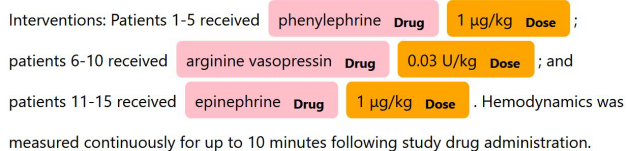
\includegraphics[width=0.8\linewidth,keepaspectratio]{spacy22}
\end{center}

\begin{columns}
    \begin{column}[T]{0.6\linewidth}
my\_config.cfg
	\begin{lstlisting}
[nlp]
lang = "en"
pipeline = ["llm"]
batch_size = 128
[components]
[components.llm]
factory = "llm"
[components.llm.model]
@llm_models = "spacy.GPT-4.v2"
[components.llm.task]
@llm_tasks = "spacy.NER.v2"
labels = ["Drug", "Dose"]
	\end{lstlisting}
    \end{column}
    \begin{column}[T]{0.4\linewidth}



my\_script.py
	\begin{lstlisting}
from spacy_llm.util import assemble
text = _read_trial(pmid=27144689)
nlp = assemble(config_path)
doc = nlp(text)
	\end{lstlisting}
\end{column}
\end{columns}




\end{frame}


%%%%%%%%%%%%%%%%%%%%%%%%%%%%%%%%%%%%%%%%%%%%%%%%%%%%%%%%%%%%%%%%%%%%%%%%%%%%%%%%%%
\begin{frame}[fragile]\frametitle{Zero-shot NER with LLMs}
\begin{columns}
\begin{column}{0.5\textwidth}
\begin{itemize}
\item Performance highly dependent on the label(s)
\begin{itemize}
\item How commonly known these types of entities are
\item How descriptive \& accurate the label text is, e.g.
\begin{itemize}
\item "Dose" vs. "TreatmentDose"
\item "Drug" vs. "Chemical" etc
\end{itemize}
\end{itemize}
\end{itemize}
\end{column}
\begin{column}{0.5\textwidth}
\begin{itemize}
\item Reproducibility can be tricky because the LLM's responses may vary
\begin{itemize}
\item For classification (not generation) tasks, you'll typically want to set temperature to 0.0
\item You can provide model-specific parameters in the config file:
\end{itemize}
\end{itemize}
\end{column}
\end{columns}

\begin{lstlisting}
[components.llm.model]
@llm_models = "spacy.GPT-4.v2"
config = {"seed": 342, "temperature": 0.0}
\end{lstlisting}

\end{frame}

%%%%%%%%%%%%%%%%%%%%%%%%%%%%%%%%%%%%%%%%%%%%%%%%%%%%%%%%%%%%%%%%%%%%%%%%%%%%%%%%%%
\begin{frame}[fragile]\frametitle{Enhancing Few-shot NER with "Chain-of-thought" Prompting}
\begin{itemize}
\item Inspired by the PromptNER paper (Ashok and Lipton, 2023)
\item LLM explains its reasoning with "tokens to think"
\item Implemented in spacy-llm as spacy.NER.v3
\item Improved F-score by 15 percentage points on internal use-case
\item Optimal performance with label definitions and examples. Allows tuning the prompt for desired results
\end{itemize}
\end{frame}

%%%%%%%%%%%%%%%%%%%%%%%%%%%%%%%%%%%%%%%%%%%%%%%%%%%%%%%%%%%%%%%%%%%%%%%%%%%%%%%%%%
\begin{frame}[fragile]\frametitle{Enhancing Few-shot NER with "Chain-of-thought" Prompting}
my\_config.cfg

\begin{lstlisting}
[components.llm.task]
@llm_tasks = "spacy.NER.v3"
labels = ["Drug", "Dose"]
description = Entities are drugs or their doses. They can be uppercased, title-cased, or 
lowercased. Each occurrence of an entity in the text should be extracted.

[components.llm.task.label_definitions]
Drug = "A medicine or drug given to a patient as a treatment. Can be a generic name or 
brand name, e.g. paracetamol, Aspirin"
Dose = "The measured quantity (dose) of a certain medicine given to patients, e.g. 1mg. 
This should exclude the drug name."

[components.llm.task.examples]
@misc = "spacy.FewShotReader.v1"
path = "my_fewshot.json"
\end{lstlisting}
\end{frame}

%%%%%%%%%%%%%%%%%%%%%%%%%%%%%%%%%%%%%%%%%%%%%%%%%%%%%%%%%%%%%%%%%%%%%%%%%%%%%%%%%%
\begin{frame}[fragile]\frametitle{Enhancing Few-shot NER with "Chain-of-thought" Prompting}
my\_fewshot.json

\begin{lstlisting}
   "text": "The patient was given 1mg of paracetamol.",
   "spans": [
     {
       "text": "paracetamol",
       "is_entity": true,
       "label": "Drug",
       "reason": "is a drug name, used as medication"
     },
     {
       "text": "1mg",
       "is_entity": true,
       "label": "Dose",
       "reason": "is the quantity or dose of the given medication"
     },
     {
       "text": "patient",
       "is_entity": false,
       "label": "==NONE==",
       "reason": "is a person, not a drug or dose"
     }
   ]
 
\end{lstlisting}
\end{frame}


%%%%%%%%%%%%%%%%%%%%%%%%%%%%%%%%%%%%%%%%%%%%%%%%%%%%%%%%%%%%%%%%%%%%%%%%%%%%%%%%%%
\begin{frame}[fragile]\frametitle{Custom Task}
\begin{columns}
\begin{column}{0.5\textwidth}
my\_task.py
	\begin{lstlisting}
INSTRUCTION = "Summarize the following clinical trial in a 
structured fashion. (...)"
@registry.llm_tasks("tutorial.TrialSummary.v1")
def make_trial_task() -> "TrialSummaryTask":
   return TrialSummaryTask(INSTRUCTION)
class TrialSummaryTask(LLMTask):
   def __init__(self, instruction: str):
       self.instruction = instruction
   def generate_prompts(self, docs):
       for doc in docs:
     yield self.instruction + "\n\n" + doc.text
 
   def parse_responses(self, docs):
	\end{lstlisting}
\end{column}
\begin{column}{0.5\textwidth}
my\_config.cfg
	\begin{lstlisting}
[nlp]
lang = "en"
pipeline = ["llm"]
batch_size = 128
[components]
[components.llm]
factory = "llm"
[components.llm.model]
@llm_models = "spacy.GPT-4.v2"
[components.llm.task]
@llm_tasks = "tutorial.TrialSummary.v1"
	\end{lstlisting}
\end{column}
\end{columns}

\end{frame}


%%%%%%%%%%%%%%%%%%%%%%%%%%%%%%%%%%%%%%%%%%%%%%%%%%%%%%%%%%%%%%%%%%%%%%%%%%%%%%%%%%
\begin{frame}[fragile]\frametitle{Output using GPT-4}
my\_fewshot.json

\begin{lstlisting}
Patient group: Group 1
Number of patients in the group: 5
Treatment drug or substance: Phenylephrine
Treatment dose: 1 $\mu$/kg
Treatment frequency of administration: Single dose
Treatment duration: Up to 10 minutes following study drug administration
Outcome: The ratio of pulmonary-to-systemic vascular resistance decreased in three of five patients. An increase in 
aortic pressure was observed.

Patient group: Group 2
Number of patients in the group: 5
Treatment drug or substance: Arginine vasopressin
Treatment dose: 0.03 U/kg
Treatment frequency of administration: Single dose
Treatment duration: Up to 10 minutes following study drug administration
Outcome: The ratio of pulmonary-to-systemic vascular resistance decreased in all five patients. An increase in aortic 
pressure was observed. Arginine vasopressin consistently resulted in a decrease in the ratio of systolic pulmonary 
artery-to-aortic pressure.

Patient group: Group 3
(...)
 
\end{lstlisting}
\end{frame}

%%%%%%%%%%%%%%%%%%%%%%%%%%%%%%%%%%%%%%%%%%%%%%%%%%%%%%%%%%%%%%%%%%%%%%%%%%%%%%%%%%
\begin{frame}[fragile]\frametitle{Post-processing LLM Output for Structured Data}

\begin{itemize}
\item The "outcome" field contains full sentences
\item Different expressions for a "single" treatment frequency:
	\begin{itemize}
	\item Administered once
	\item Single administration
	\item One-time dose
	\item One time
	\item Single dose
	\item One-time administration
	\item Once
	\end{itemize}
\item Post-processing of results is still required to obtain structured fields
\end{itemize}

\end{frame}

%%%%%%%%%%%%%%%%%%%%%%%%%%%%%%%%%%%%%%%%%%%%%%%%%%%%%%%%%%%%%%%%%%%%%%%%%%%%%%%%%%
\begin{frame}[fragile]\frametitle{From text to structured data: a pipeline approach}

\begin{center}
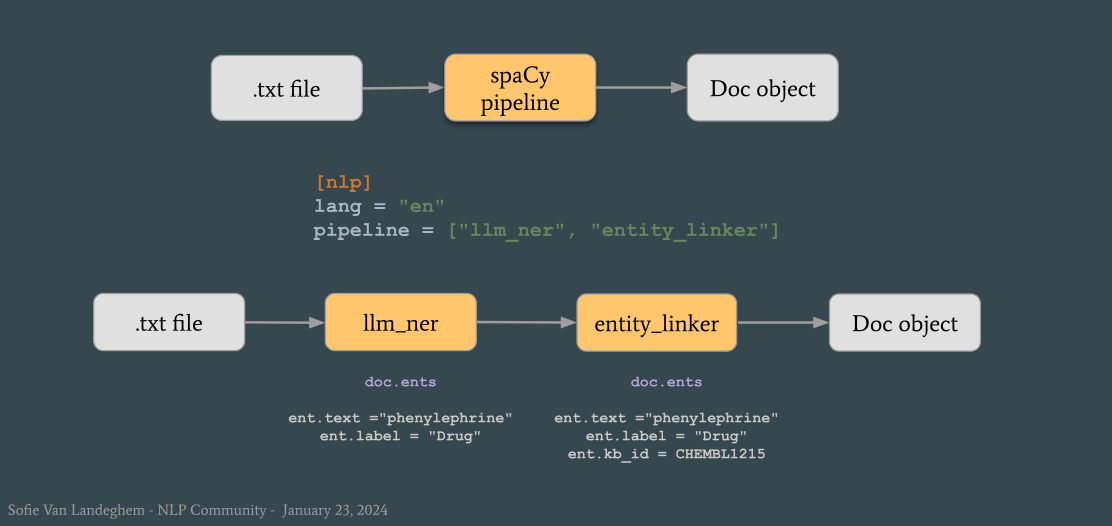
\includegraphics[width=\linewidth,keepaspectratio]{spacy23}
\end{center}


\end{frame}


%%%%%%%%%%%%%%%%%%%%%%%%%%%%%%%%%%%%%%%%%%%%%%%%%%%%%%%%%%%%%%%%%%%%%%%%%%%%%%%%%%
\begin{frame}[fragile]\frametitle{From a trial text to structured output}

\begin{center}
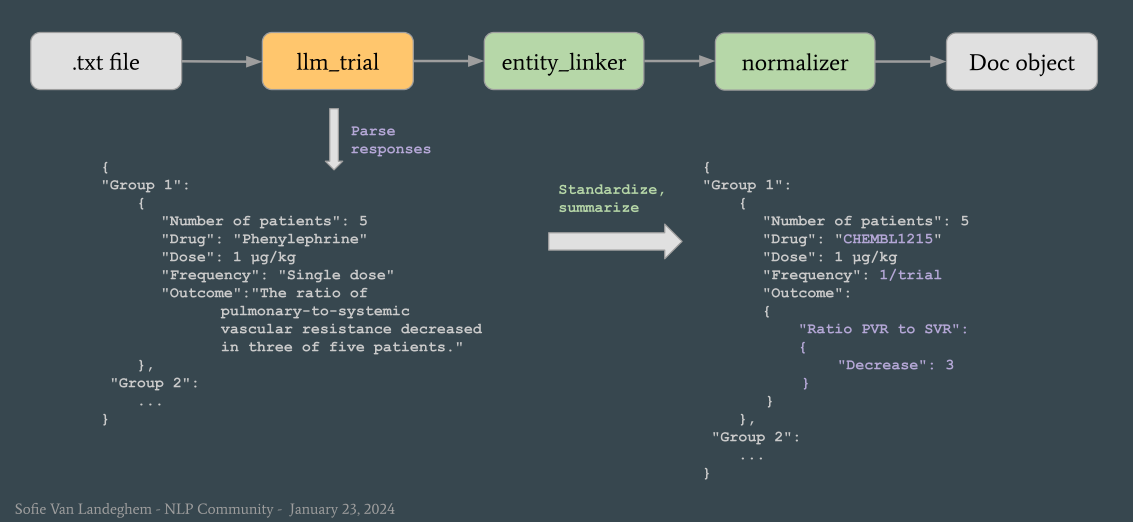
\includegraphics[width=\linewidth,keepaspectratio]{spacy24}
\end{center}


\end{frame}

%%%%%%%%%%%%%%%%%%%%%%%%%%%%%%%%%%%%%%%%%%%%%%%%%%%%%%%%%%%%%%%%%%%%%%%%%%%%%%%%%%
\begin{frame}[fragile]\frametitle{Swap out the LLM backend}

\begin{center}
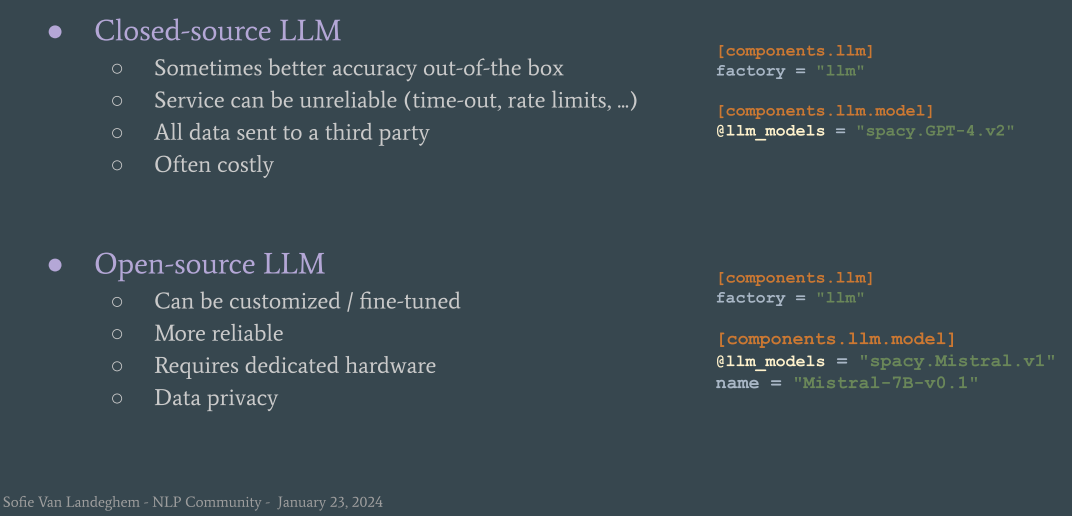
\includegraphics[width=\linewidth,keepaspectratio]{spacy25}
\end{center}


\end{frame}

%%%%%%%%%%%%%%%%%%%%%%%%%%%%%%%%%%%%%%%%%%%%%%%%%%%%%%%%%%%%%%%%%%%%%%%%%%%%%%%%%%
\begin{frame}[fragile]\frametitle{Swap out a component architecture}

\begin{center}
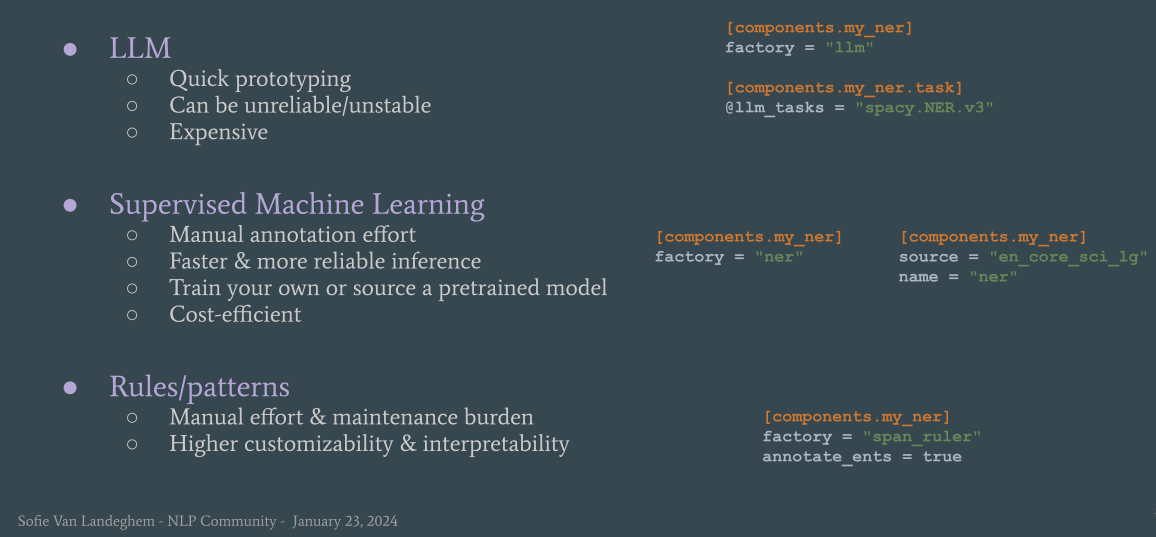
\includegraphics[width=\linewidth,keepaspectratio]{spacy26}
\end{center}


\end{frame}

%%%%%%%%%%%%%%%%%%%%%%%%%%%%%%%%%%%%%%%%%%%%%%%%%%%%%%%%%%%%%%%%%%%%%%%%%%%%%%%%%%
\begin{frame}[fragile]\frametitle{Combine the best of both worlds (example)}

\begin{center}
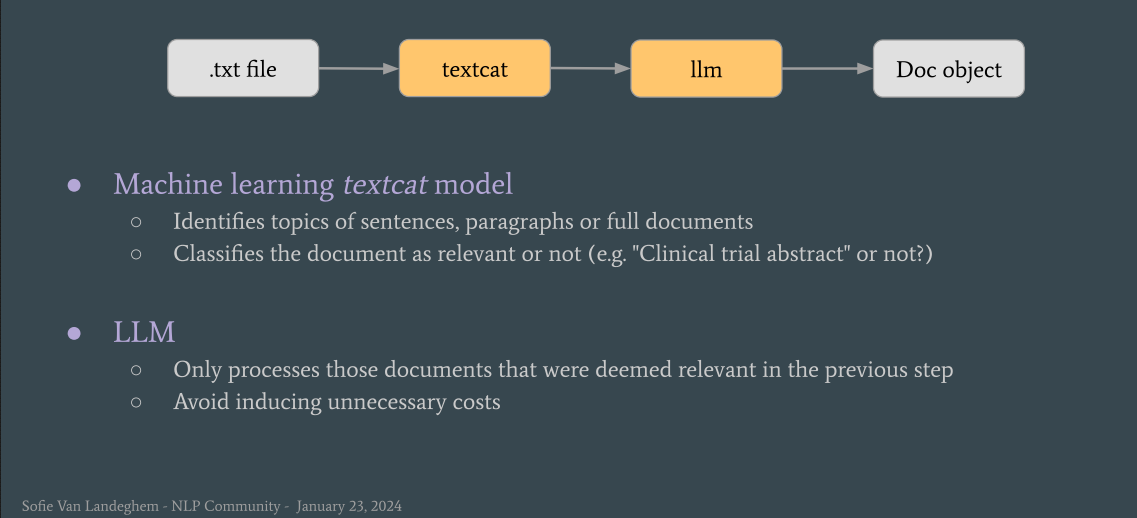
\includegraphics[width=\linewidth,keepaspectratio]{spacy27}
\end{center}


\end{frame}

%%%%%%%%%%%%%%%%%%%%%%%%%%%%%%%%%%%%%%%%%%%%%%%%%%%%%%%%%%%%%%%%%%%%%%%%%%%%%%%%%%
\begin{frame}[fragile]\frametitle{The Importance of Annotations}

	\begin{itemize}
	\item Evaluation
	\begin{itemize}
	\item Required for representative evaluation set
	\item Measure single component performance
	\item Measure end-to-end pipeline performance
	\item Track progress during pipeline changes
	\end{itemize}
	\item Training supervised models
	\begin{itemize}
	\item Smaller, specialized models can be cost-efficient
	\end{itemize}
	\item Tuning LLMs
	\begin{itemize}
	\item Provide "difficult" examples for few-shot prompts
	\item Perform fine-tuning on LLM
	\end{itemize}
	\end{itemize}

\end{frame}

%%%%%%%%%%%%%%%%%%%%%%%%%%%%%%%%%%%%%%%%%%%%%%%%%%%%%%%%%%%%%%%%%%%%%%%%%%%%%%%%%%
\begin{frame}[fragile]\frametitle{LLM-assisted annotation (NER)}

\begin{center}
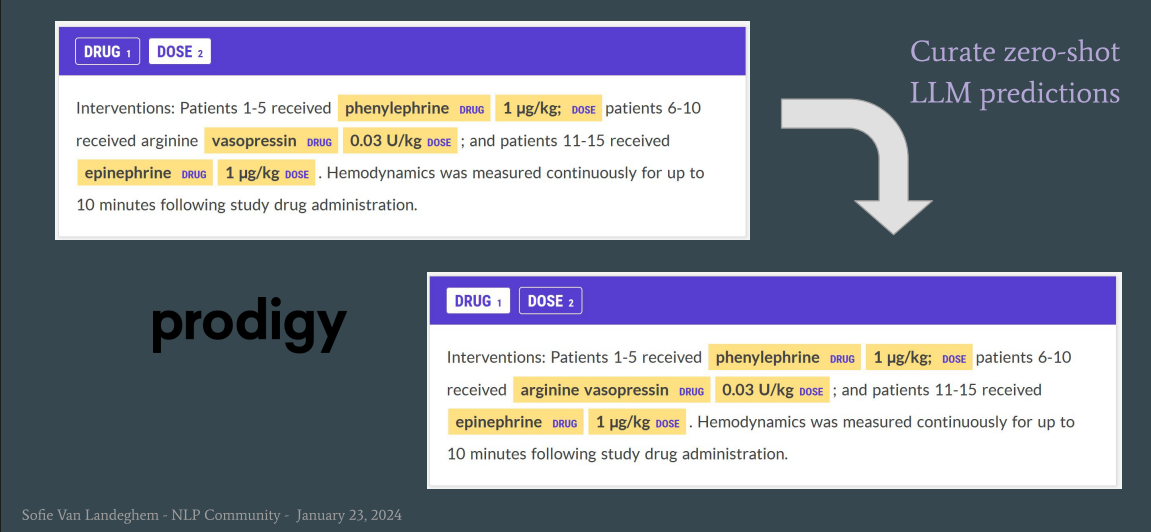
\includegraphics[width=\linewidth,keepaspectratio]{spacy28}
\end{center}


\end{frame}

%%%%%%%%%%%%%%%%%%%%%%%%%%%%%%%%%%%%%%%%%%%%%%%%%%%%%%%%%%%%%%%%%%%%%%%%%%%%%%%%%%
\begin{frame}[fragile]\frametitle{LLM-assisted annotation (REL)}

\begin{center}
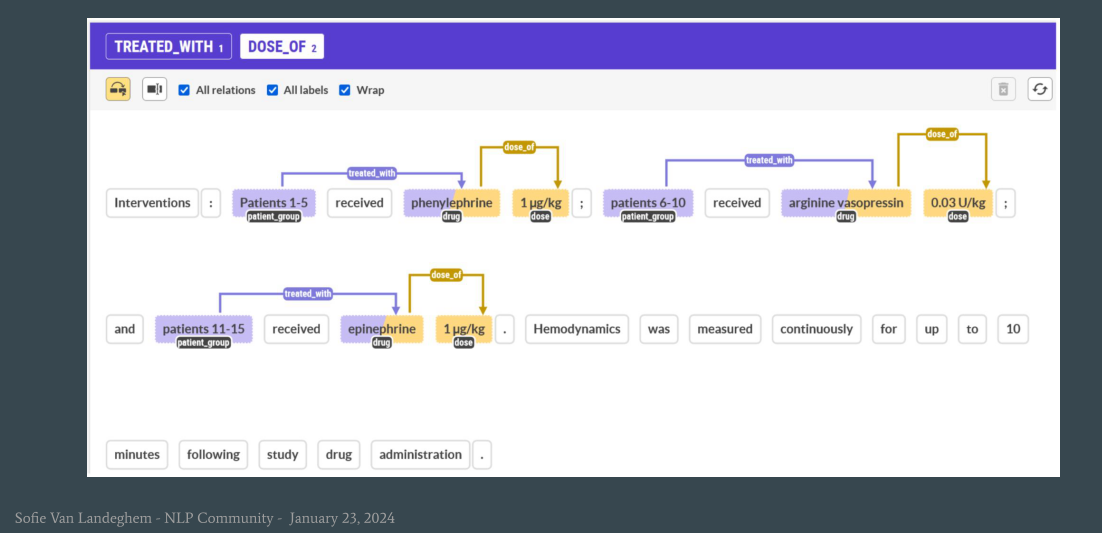
\includegraphics[width=\linewidth,keepaspectratio]{spacy29}
\end{center}


\end{frame}

%%%%%%%%%%%%%%%%%%%%%%%%%%%%%%%%%%%%%%%%%%%%%%%%%%%%%%%%%%%%%%%%%%%%%%%%%%%%%%%%%%
\begin{frame}[fragile]\frametitle{Summary}
\begin{itemize}
\item LLMs are great for quick prototyping and bootstrapping annotation
\item NLP solutions balance accuracy, reliability, maintainability, customizability, and cost
\begin{itemize}
\item Mix and match LLMs with supervised models or rule-based components
\item spaCy pipelines are versatile
\item Easily swap out components while keeping others in the pipeline
\end{itemize}
\item spacy-llm facilitates LLM integration into structured NLP pipelines
\begin{itemize}
\item Swap between closed-source LLMs (API) and open-source ones
\item Use built-in standard NLP tasks
\item Write custom tasks, fine-tune prompts, etc.
\end{itemize}
\end{itemize}
\end{frame}